\begin{figure}
  \centering
  % http://pgfplots.sourceforge.net/gallery.html
  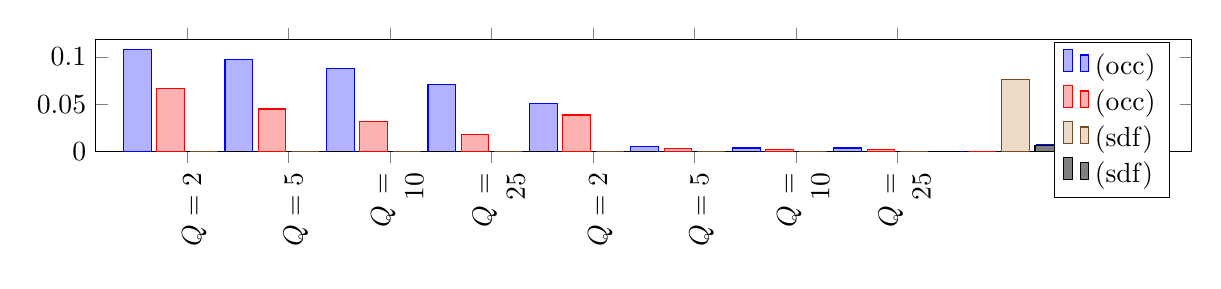
\begin{tikzpicture}
    \begin{axis}[
        ybar,
        % https://tex.stackexchange.com/questions/119887/remove-the-scientific-notation-which-is-unreasonable
        yticklabel style={
          /pgf/number format/fixed,
          /pgf/number format/precision=5
        },
        scaled y ticks=false,
        %legend style={
        %  at={(1.05,1)},
        %  anchor=north west,
        %},
        % https://tex.stackexchange.com/questions/48620/pgfplots-alignment-and-size-of-math-in-legend
        legend cell align=left,
        % https://tex.stackexchange.com/questions/135595/how-to-correct-problem-with-ybar-plot-bad-axis-and-too-many-labels-in-x-axis
        xtick={
          1, 2, 3, 4,
          5, 6, 7, 8
        },
        xticklabels={
          \PPCA\\$Q = 2$, \PPCA\\$Q = 5$, \PPCA\\$Q = 10$, \PPCA\\$Q = 25$,
          \VAE\\$Q = 2$, \VAE\\$Q = 5$, \VAE\\$Q = 10$, \VAE\\$Q = 25$,
        },
        x tick label style={text width=1cm,align=right},
        ymin=0,
        height=3cm,
        width=15.5cm,
        % https://tex.stackexchange.com/questions/271027/pgfplots-how-to-rotate-extra-x-tick-labels
        x tick label style={
          rotate=90,
          anchor=east,
        },
      ]
        
      % Abs
      \addplot coordinates {
        (1, 0.107466870529)
        (2, 0.0973753175757)
        (3, 0.0876120861329)
        (4, 0.0711613035139)
        (5, 0.05121126)
        (6, 0.00515391)
        (7, 0.00361275)
        (8, 0.00366516)
        (9, 0)
        (10, 0.00777563)
      };
      \addlegendentry{\Abs (occ)}
      % AbsThr
      \addplot coordinates {
        (1, 0.06709765625)
        (2, 0.0449326171875)
        (3, 0.0312314453125)
        (4, 0.0177939453125)
        (5, 0.03853159)
        (6, 0.00318352)
        (7, 0.00182621)
        (8, 0.00181555)
        (9, 0)
        (10, 0.00499229)
      };
      \addlegendentry{\AbsThr (occ)}
      %
      \addplot coordinates {
        (1, 0)
        (2, 0)
        (3, 0)
        (4, 0)
        (5, 0)
        (6, 0)
        (7, 0)
        (8, 0)
        (9, 0.07644901)
        (10, 0.07105859)
      };
      \addlegendentry{\Abs (sdf)}
      %
      \addplot coordinates {
        (1, 0)
        (2, 0)
        (3, 0)
        (4, 0)
        (5, 0)
        (6, 0)
        (7, 0)
        (8, 0)
        (9, 0.00623527)
        (10, 0.00514245)
      };
      \addlegendentry{\AbsThr (sdf)}
    \end{axis}
  \end{tikzpicture}
  % TODO short caption
  \caption{Absolute error \Abs and absolute error on thresholded reconstructions
  \AbsThr for \PPCA with different size $Q \in \{2,5,10,25\}$ of the latent space.}
  \label{fig:experiments-2d-ppca}
\end{figure}
